\documentclass[dvipdfmx,autodetect-engine,twocolumn,10pt]{jsarticle}% autodetect-engine で pLaTeX / upLaTeX を自動判定
\setlength{\columnsep}{3zw}
\usepackage[dvipdfmx]{graphicx}
\usepackage{amsmath,amssymb}

\title{モンテカルロ法による光子輸送シミュレーションと\\
3次元画像のモンテカルロシミュレーション}
\author{法政大学理工学部 応用情報工学科 4年 16X3128 馬場俊弥}
\date{2019年5月25日}

\begin{document}

\maketitle
\section{モンテカルロ法による光子輸送シミュレーション}
モンテカルロ法とは,シミュレーションや数値計算を乱数を用いて反復計算を行うことにより,確率的に問題の解を推定する方法である.
1個の光子輸送のフローチャートを図\ref{photon_flow}に示す.

\begin{figure}[h]
  \begin{center}
    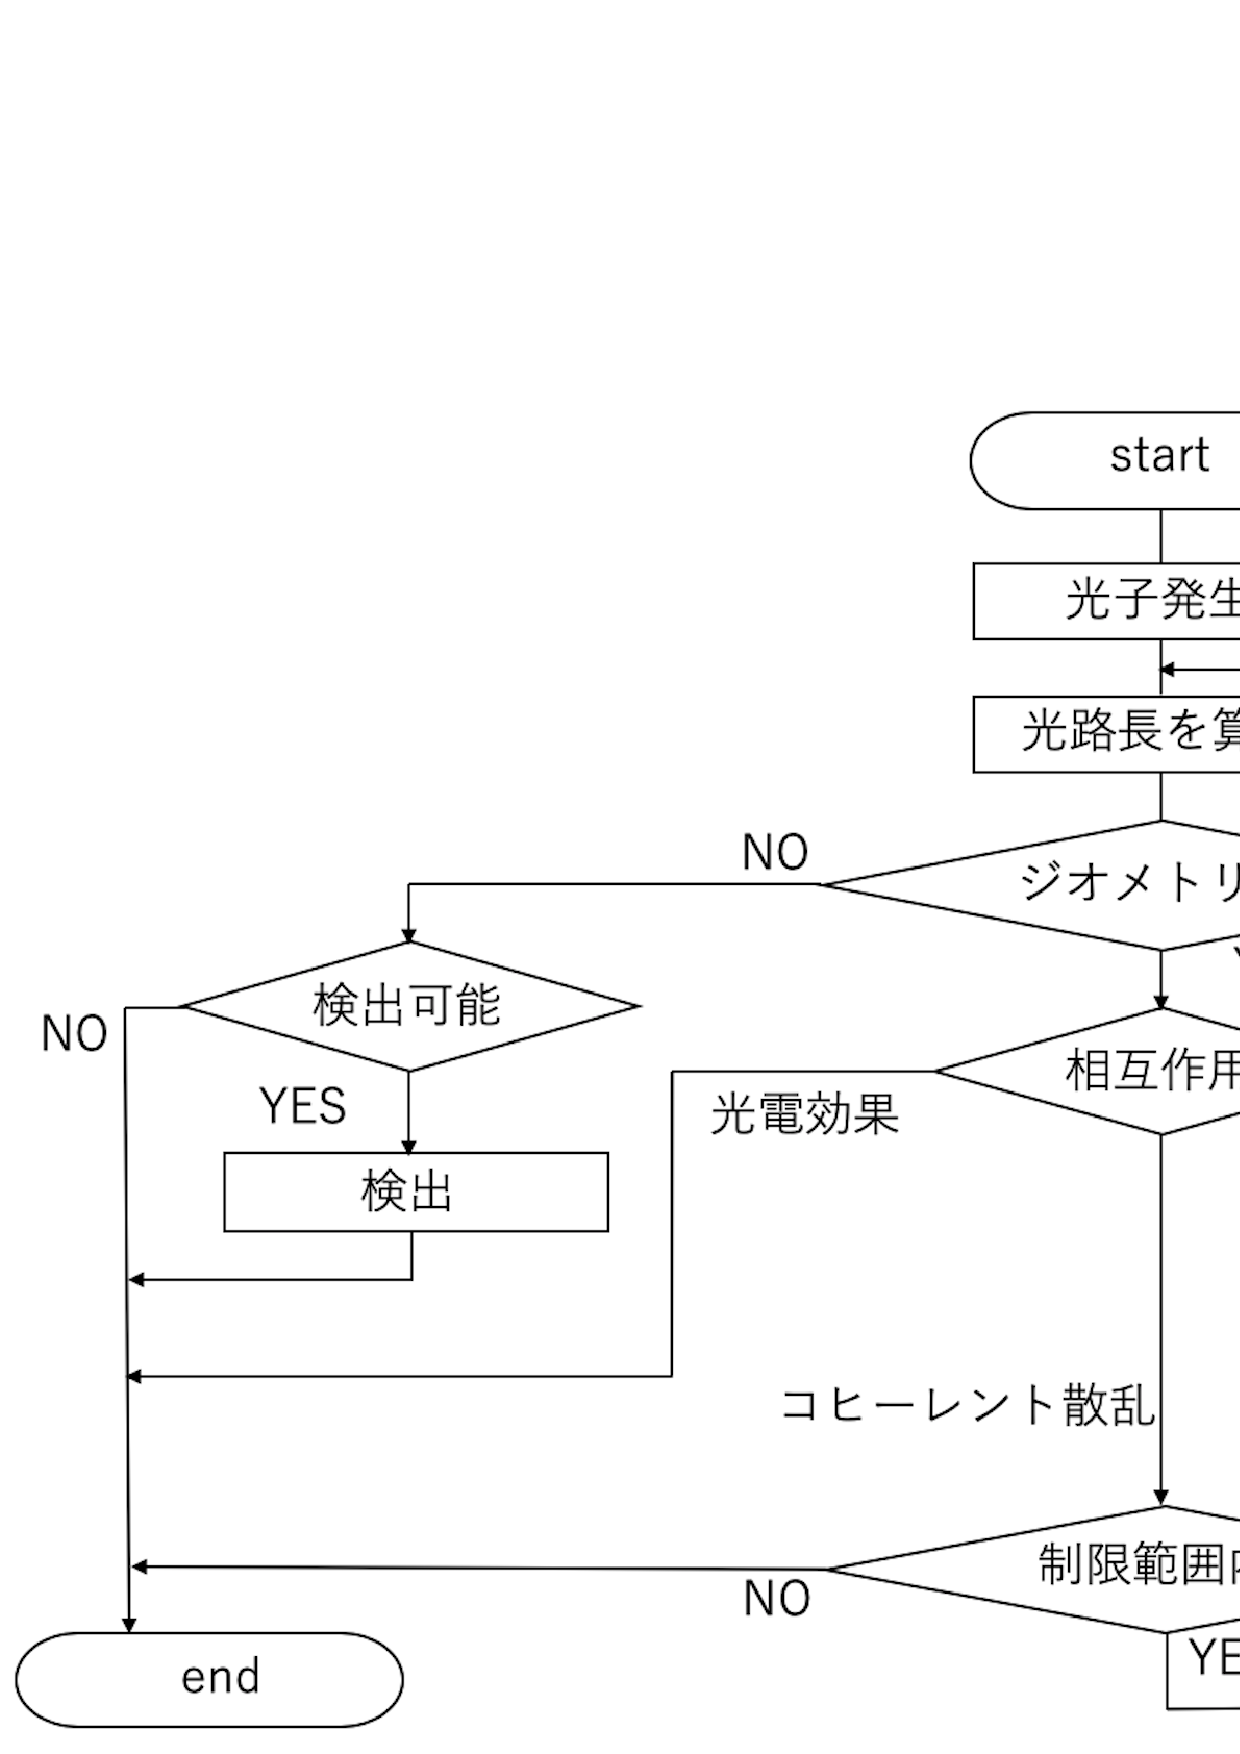
\includegraphics[width=7cm]{./file/monte_simu_flow.png}\\
    \caption{光子輸送のフローチャート}
    \label{photon_flow}
  \end{center}
\end{figure}

図1のように,光子は相互作用を引き起こす.今回のシミュレーションではコンプトン散乱,コヒーレント散乱,光電効果の3つの相互作用を考慮する.(コヒーレント,コンプトン,光電効果の説明を入れる)

\section{3次元画像のモンテカルロシミュレーション}


\section{シミュレーション}
\subsection{モンテカルロ法による光子輸送シミュレーション}
シミュレーション条件を表\ref{simu_cond}に示す.
\begin{table}[htb]
  \begin{center}
    \caption{シミュレーション条件}
    \label{simu_cond}
    \begin{tabular}{|c|c|} \hline
      媒質 & $H_2O$ \\ \hline
      初期エネルギー & 140 KeV \\ \hline
      光子数 & 1億個 \\ \hline
      最大散乱回数 & 5回 \\ \hline
      光子の初期位置 & 原点 \\ \hline
      光子の放出方向 & z軸正方向 \\ \hline
      検出器のサイズ & 65×65 pixel \\ \hline
      カットオフエネルギー & 30 KeV \\ \hline
    \end{tabular}
  \end{center}
\end{table}
\subsection{3次元画像のモンテカルロシミュレーション}
表でシミュレーション条件(水)

\section{結果}
\subsection{モンテカルロ法による光子輸送シミュレーション}
各散乱回数毎の結果画像とそのプロファイルをそれぞれ図\ref{monte_result}に示す.

\begin{figure}[ht]
  \begin{center}
    \begin{tabular}{c}
      \begin{minipage}{0.5\hsize}
        \begin{center}
          
\includegraphics[clip, width=2cm]{./file/monte_simu_primary.eps}
          \hspace{0.5cm} [a]散乱回数0回
        \end{center}
      \end{minipage}

      \begin{minipage}{0.5\hsize}
        \begin{center}
          
\includegraphics[clip, width=2cm]{./file/monte_simu_1.eps}
          \hspace{0.5cm} [b]散乱回数1回
        \end{center}
      \end{minipage}
    \caption{各散乱回数毎の結果画像}
    \label{monte_result}
  \end{center}
\end{figure}

% \begin{figure}[ht]
%   \begin{center}
%     
\includegraphics[clip, width=2cm]{./file/monte_simu_primary.eps}
%     \caption{各散乱回数毎の結果画像}
%     \label{monte_result}
%   \end{center}
% \end{figure}

\subsection{3次元画像のモンテカルロシミュレーション}
投影画像と再構成結果(MLなしML50回)

\section{理論値との比較}
光子輸送シミュレーションを比較する.

\section{まとめと今後の展望}




\end{document}
